\chapter{IETF Standards}
\label{IETF}
The constraints presented in Section~\ref{General:WSN} and the difficulties in combining IPv6 with WSN are significant. To realize it, the various working groups of IETF have proposed a series of standards in order to solve the problems.

\section{Adaptation Layer: 6LoWPAN}
\label{Intr:6LoWPAN}
The IETF introduced an IPv6 over Low power Wireless Personal Area Networks (6LoWPAN) model, which allows for IPv6 packets to be transmitted or received by the IEEE 802.15.4 network. The detailed specification can be found in~\cite{RFC 4944}.

Instead of the traditional IP based model, a 6LoWPAN protocol stack adds the 6LoWPAN adaptation layer under the IP network layer. Figure~\ref{fig:node stack} shows the protocol stacks of a typical 6LoWPAN node and the protocol stack for the 6LBR is shown in Figure~\ref{fig:6LBR stack}.

\begin{figure}[htbp]
  \begin{center}
    \leavevmode
    \subfloat[Typical 6LoWPAN Node]{\label{fig:node stack}
      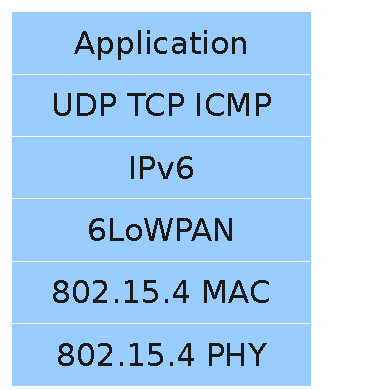
\includegraphics[scale=0.5]{Pics/Protocol.pdf}}
    \subfloat[6LBR]{\label{fig:6LBR stack}
       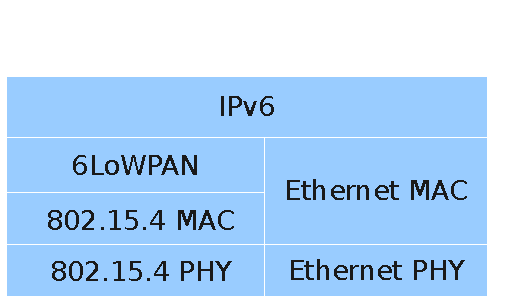
\includegraphics[scale=0.5]{Pics/6LBR.pdf}}
    \caption{Protocol stack of 6LoWPAN nodes}
    \label{fig:protocol stack}
  \end{center}
\end{figure}
\index{figure 3.1}

A 6LBR is a network layer router; when packets are routed though the 6LBR to an external IPv6 based network, the adaptation layer in the LBR translates the LoWPAN format header into a full IPv6 format, and
vice versa. In some practical applications, the adaptation layer is implemented along with an IP
layer such as, for example, in the 6LoWPAN implementation BLIP.

In the adaptation layer, IPv6 header compression and data fragmentation will be performed to solve the problem of frame size incompatibility, and along with layer-two forwarding~\texttt{mesh-under}, it would allow IPv6 packets to be transmitted via the 802.15.4 network. The basic 6LoWPAN frame structure is shown in Figure~\ref{fig:Frame}.  

\begin{figure}[htbp]
  \begin{center}
    \leavevmode
    %\framebox{
     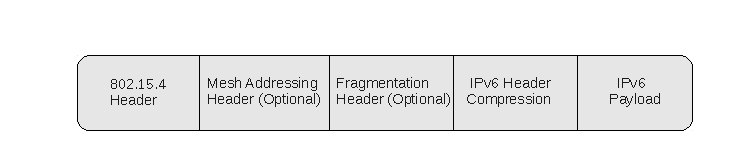
\includegraphics[scale=1]{Pics/Frame.pdf}%}
    \caption{The basic 6LoWPAN frame structure}
    \label{fig:Frame}
  \end{center}
\end{figure}
\index{figure 3.2}

\subsection{Header Compression}
\label{IETF:HC}
The first scheme performed is IPv6 header compression. The idea is to eliminate the
header which contains information of the 6LoWPAN network. There are two compression formats: header compression one (HC1) and header compression two (HC2)\@. HC1 and HC2 are respectively responsible for the IPv6 header and transport protocol header.  First, the HC1 reduces the 40 octets IPv6 overhead into 2 octets (1 octet for the HC1 encoding and 1 octet for the hop limit)\@. The HC2 is then used to compress any overhead brought by transport layer protocols such as, for example, UDP, TCP, or ICMP.

\subsection{Packet Fragmentation}
\label{IETF:PF}

\begin{figure}[htbp]
  \begin{center}
    \leavevmode
    %\framebox{
    \subfloat[First Fragment]{\label{fig:Fragmentation_1}
      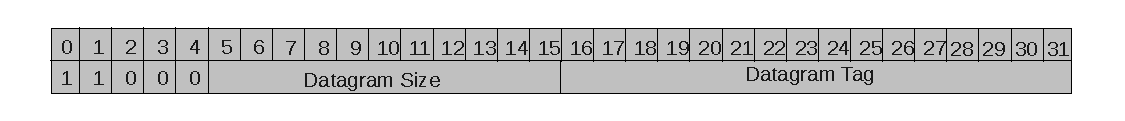
\includegraphics[scale=0.8]{Pics/Fragmentation_1.pdf}}\\
    \subfloat[Subsequent Fragment]{\label{fig:Fragmentation_2}
       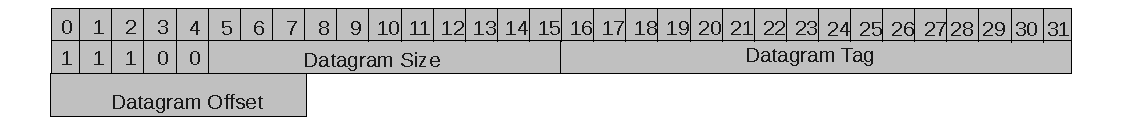
\includegraphics[scale=0.8]{Pics/Fragmentation_2.pdf}}
    \caption{Fragmentation header of 6LoWPAN}
    \label{fig:Fragmentation}
  \end{center}
\end{figure}
\index{figure 3.3}

In front of the compressed IPv6 header there is a fragmentation header (Figure~\ref{fig:Frame})\@. This fragmentation header is only introduced when an IPv6 payload does not fit into a single IEEE 802.15.4 frame;
the payload then needs to be fragmented into several packets. It is used in order to indicate the proper order of the sequences. Figure~\ref{fig:Fragmentation_1} gives the header format for the first
fragment; the header format for subsequent fragments is given in Figure~\ref{fig:Fragmentation_2}.

When using the routing mechanism~\texttt{mesh-under} (in contrast to~\texttt{route-over}, which forwards packets using IP layer addresses)\@, a mesh addressing header precedes the fragmentation header. Because the source and destination addresses in IPv6 headers are compressed in header compression, this mesh addressing header is needed for packets to be correctly forwarded in a layer-two fashion. The mesh addressing header format with short 16-bit link layer addresses is shown in Figure~\ref{fig:Mesh} (the mesh addressing header with EUI 64-bit addresses has the same format)\@. The first bit and second bit indicates that this header is mesh type. The V bit indicates the originator address (V in this case stands for Very First) being a short 16-bit or an EUI 64-bit address, while F (for Final) bit represents that of the destination address.  This is then followed by a 4-bit section which indicates the numbers of hops remaining and, finally, the link layer addresses for source and destination are added.
\begin{figure}[htbp]
  \begin{center}
    \leavevmode
    %\framebox{
      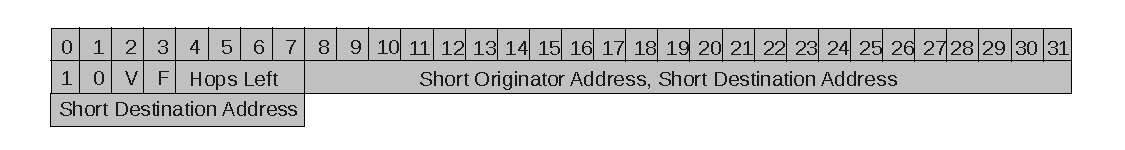
\includegraphics[scale=0.8]{Pics/Mesh.pdf}%}
    \caption{Mesh addressing header of 6LoWPAN}
    \label{fig:Mesh}
  \end{center}
\end{figure}
\index{figure 3.4}

\section{Routing Protocol for Low power and Lossy Networks}
\label{RPL}
IPv6 Routing Protocol for Low power and lossy networks (RPL) as a mesh routing protocol was described by IETF in~\cite{draft-ietf-roll-rpl-19}. RPL is designed to meet the requirements such as: routing requirements for urban (\cite{RFC 5548})\@, industrial (\cite{RFC 5673})\@, home automation (\cite{RFC 5826}) and building automation (\cite{RFC 5867}) usages\@. In RPL the routing objectives, such as minimizing energy, minimize latency, etc., are separately defined in Objective Functions (OFs)\@. It makes RPL flexible to a wider range of Low power and Lossy Networks (LLNs)\@.

\subsection{Topology}
\label{RPL:Topology}

\begin{figure}[htbp]
  \begin{center}
    \leavevmode
      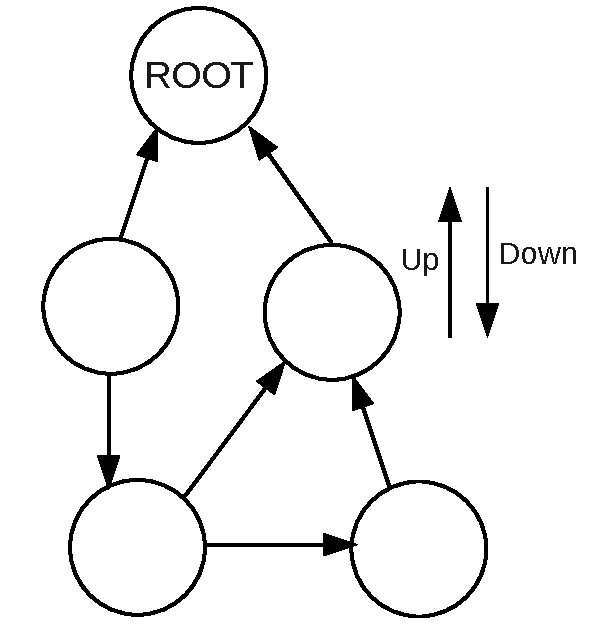
\includegraphics[scale=0.4]{Pics/DODAG.pdf}
    \caption{DODAG}
    \label{fig:DODAG}
  \end{center}
\end{figure}
\index{figure 3.5}
The most basic routing topology RPL forms and maintains is a Destination Oriented Directed Acyclic Graph (DODAG)\@. Figure~\ref{fig:DODAG} shows how a DODAG would look like: it consists of only one root node and has no loop back cycles. There are two directions defined - up which indicates the path towards the root; down which indicates the path away from the root. In a DODAG, a parent of a node is one of the immediate successors of the node on a path towards the DODAG root~\cite{draft-ietf-roll-rpl-19}. 

Four types of identifier are used in RPL:
\begin{itemize}
\item RPLInstanceID: Identifier of a RPL instance which defined as a set of one or more DODAGs with the same OF.


\item DODAGID: unique ID for each DODAG in a RPL instance.


\item DODAGVersionNumber: ID for each version of a constructed DODAG. Figure~\ref{fig:DODAGVersion} shows an example of a DODAG version change.

\item Rank: a scalar representation of the relative node position with respect to the DODAG root in a DODAG version. 
The rank of a DODAG parent should be lower than that of a child. Rank helps RPL nodes to detect loops and verify forward progression toward the destination. An simple example is shown in Figure~\ref{fig:Rank}.
\end{itemize}

\begin{figure}[htbp]
  \begin{center}
    \leavevmode
      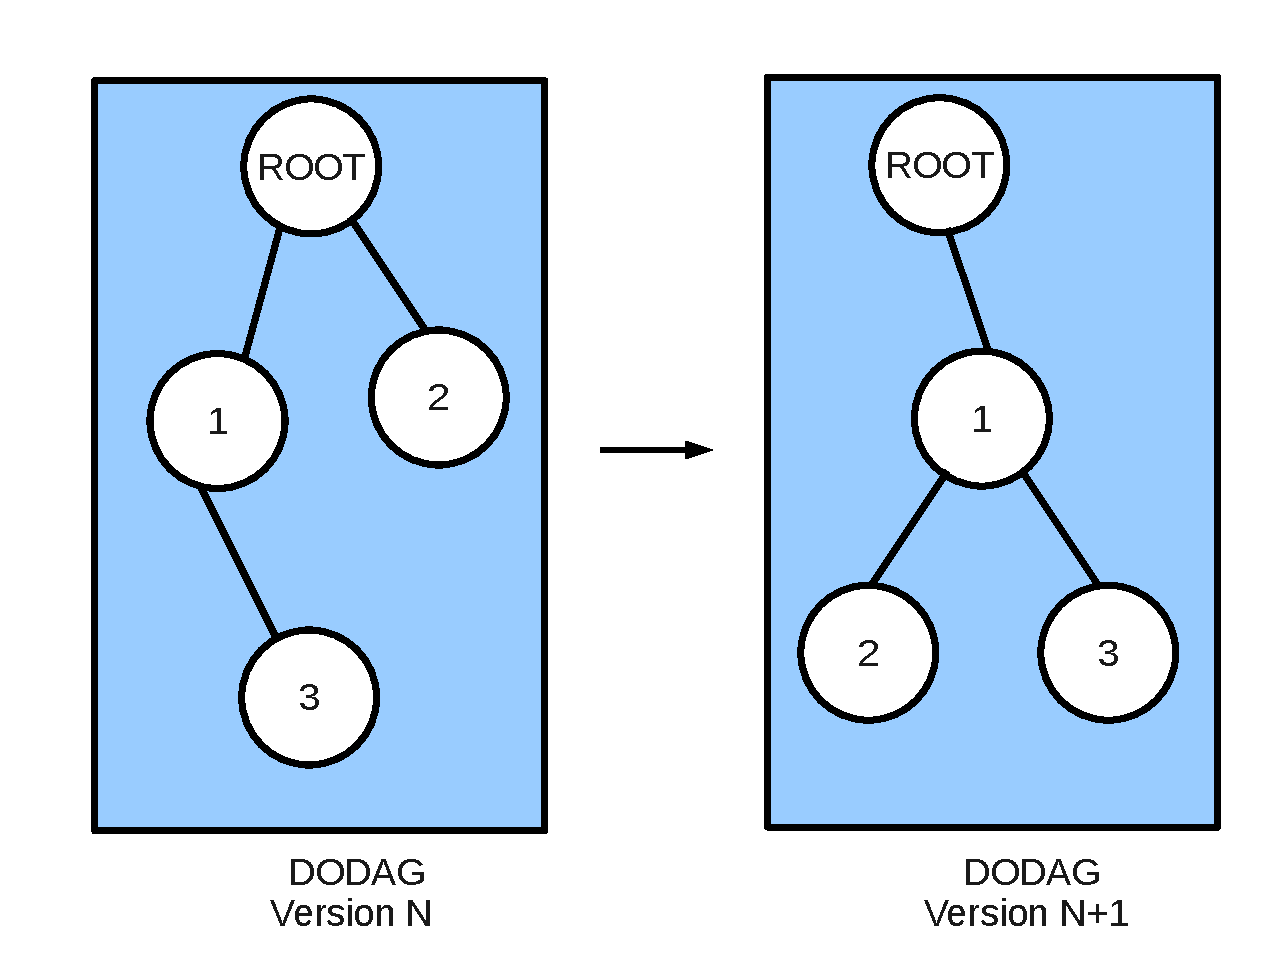
\includegraphics[scale=0.3]{Pics/DODAGVersion.pdf}
    \caption{Node 2 decides to choose node 1 as its parent instead of root which causes a DODAG reconstruction, thus the DODAG version changes.}
    \label{fig:DODAGVersion}
  \end{center}
\end{figure}
\index{figure 3.6}

\begin{figure}[htbp]
  \begin{center}
    \leavevmode
      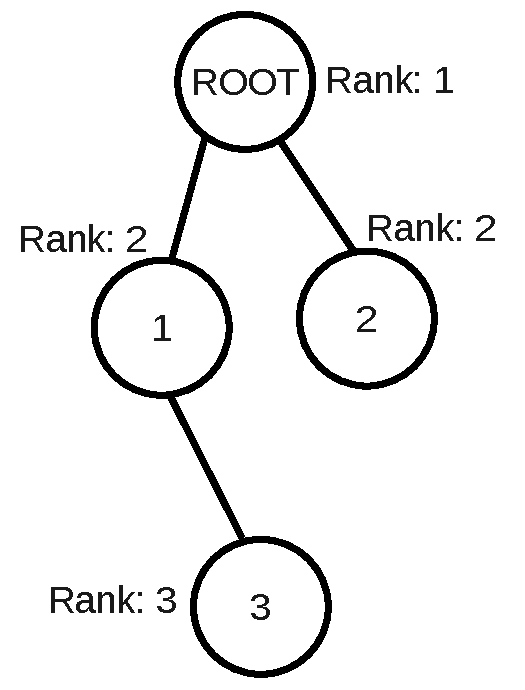
\includegraphics[scale=0.35]{Pics/Rank.pdf}
    \caption{Node 3 has a higher rank than node 1 and 2, meaning that node 3 is further from the root node than node 1 and 2.}
    \label{fig:Rank}
  \end{center}
\end{figure}
\index{figure 3.7}

The pair of RPLInstanceID and DODAGID defines a unique DODAG, Figure~\ref{fig:InstanceID} illustrates the relationship between RPL instance and DODAGs. 
The triple of RPLInstanceID, DODAGID and RPLVersionNumber uniquely identifies a DODAG version.

\begin{figure}[htbp]
  \begin{center}
    \leavevmode
      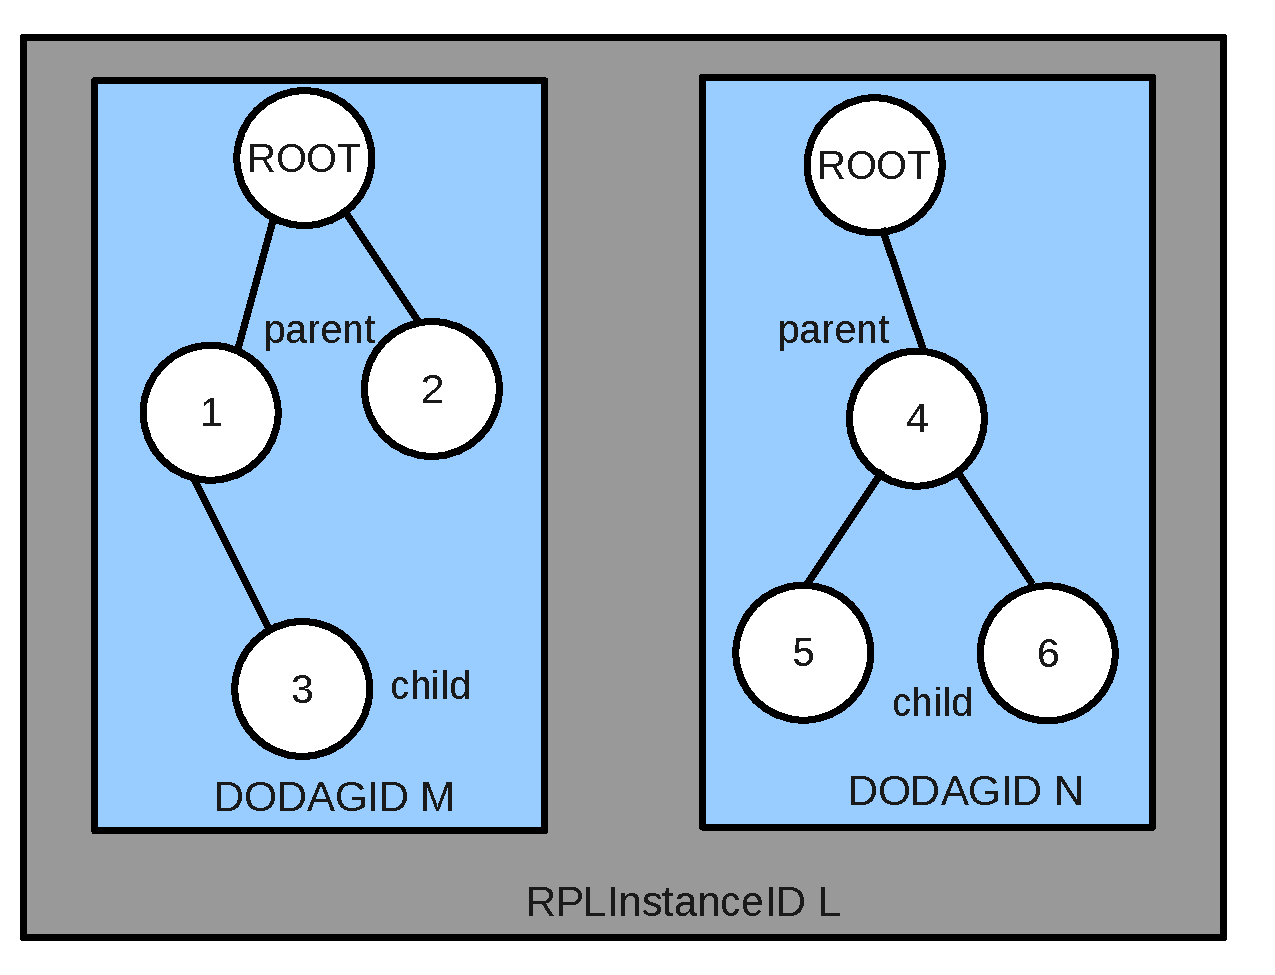
\includegraphics[scale=0.25]{Pics/InstanceID.pdf}
    \caption{A single RPL instance L includes two DODAGs with DODAGID M and N.}
    \label{fig:InstanceID}
  \end{center}
\end{figure}
\index{figure 3.8}

\subsection{ICMPv6 Control Messages for RPL}
\label{RPL:ICMP}

As the DODAG has two directions - up and down, there are two kinds of routes defined in RPL: upward routes and downward routes. Upward routes are the routes from a child node to a root node. Similarly, downward routes are the routes which are away from the root to a child node. To maintain these routes, five new types of ICMPv6 control messages are used:

\begin{itemize}
\item DODAG Information Solicitation (DIS): DIS is used by a non-root node to request DODAG information from the neighboring nodes. The neighbors respond to a DIS with a DODAG Information Object (DIO) which is the second type of ICMPv6 message used in RPL.

\item DODAG Information Object (DIO): Information such as node rank, RPL instance ID, DODAG version number are communicated between nodes within DIO messages. It allows the recipient to join a DODAG and choose its parent set and preferable parent according to the OF, routing metrics and constraints which are carried in a metric container. The sending of DIO can be triggered by both a Trickle timer or receiving a DIS.

\item Destination Advertisement Object (DAO): DAO is typically unicasted by a non-root node to its DAO parent in order to discover and maintain downward routes. DAO sending will be triggered in case of receiving a DIO or receiving a DAO message which is considered new by the recipient.

\item Destination Advertisement Object Acknowledgement (DAO-ACK): The DAO-ACK message is unicasted by recipient to acknowledge the receiving of the unicast DAO.

\item Consistency Check (CC): This message protects against replay attacks and synchronize counters. It is related to the secured RPL transmission.
\end{itemize}

Figure~\ref{fig:DIS/DIO/DAO} shows the basic DIS-DIO and DAO message exchanges. In Figure~\ref{fig:seqence_shot_DIO}, a RPL node sends a DIS to its neighbor and the neighbor will reply with a DAO message. In Figure~\ref{fig:seqence_shot_DAO}, a child sends a DAO message upwards to its parent, and the parent forwards the message to its parent until it reaches the DADAG root.  

\begin{figure}[htbp]
  \begin{center}
    \leavevmode
    %\framebox{
    \subfloat[DIS-DIO]{\label{fig:seqence_shot_DIO}
      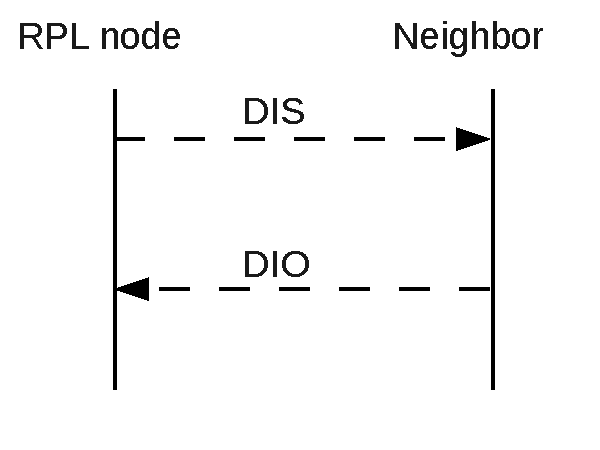
\includegraphics[scale=0.35]{Pics/DIS_DIO.pdf}}\\
    \subfloat[DAO]{\label{fig:seqence_shot_DAO}
       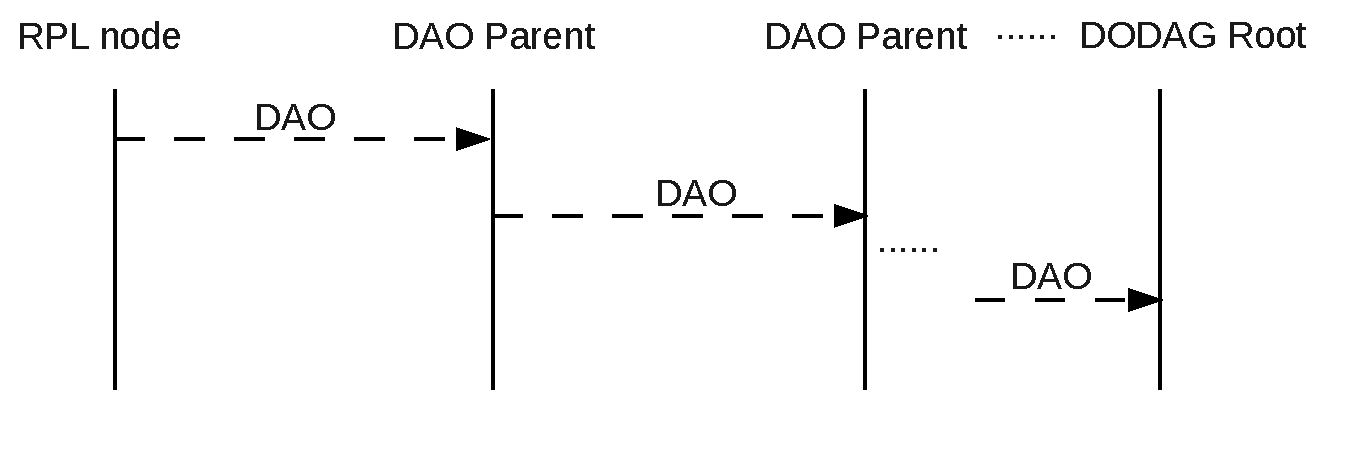
\includegraphics[scale=0.35]{Pics/DAO.pdf}}
    \caption{Basic DIS, DIO and DAO communication}
    \label{fig:DIS/DIO/DAO}
  \end{center}
\end{figure}
\index{figure 3.9}

\subsection{RPL Objective Function}
\label{RPL:OF}
An Objective Function (OF) in RPL is the function which governs route selection. It does so by using a number of metrics which describe a link or a node. These metrics are advertised in DIO messages using a Metric Container option. An OF uses these metrics to calculate rank, choose parents and therefore choose routes~\cite{MRHOF}. The actual algorithms for rank calculation parent choosing are implementation-dependent.

\subsubsection{Objective Function Zero}
\label{RPL:OF0}
The Objective Function Zero (OF0) is a very basic type of OF defined in~\cite{draft-ietf-roll-of0-20}. There is no guarantee that the chosen route is the result of applying a specific metric. Currently 0F0 is the default OF in RPL.
 
\subsubsection{The Minimum Rank Objective Function with Hysteresis}
\label{RPL:MRHOF}
The Minimum Rank Objective Function with Hysteresis (MRHOF)\@, is designed to find the paths with the smallest path cost. It does so by finding the minimum cost path and switching to that path only if it is shorter (in terms of path cost) than the current path by at least a given threshold~\cite{MRHOF}. 

The path cost in MRHOF is defined as the quantitated property of an end-to-end path, and is obtained by summing up the selected metric of the links or nodes along the path. If a DIO doesn't advertise a metric container, MRHOF uses the expected transmission count metric (ETX) as its metric. The ETX metric allows RPL to find the stable minimum-ETX paths from the nodes to a root in the DODAG instance~\cite{MRHOF}. The rank of a node in MRHOF is directly associated with the path cost of the worst parent in the parent set.

\section{RPL Control Message Timer - the Trickle Timer}
\label{Trickle}
In Section~\ref{RPL:ICMP}, the Trickle timer is mentioned as the control timer for sending DIOs. The Trickle timer uses the Trickle algorithm (\cite{RFC 6206}) to regulate control messages sending. The general idea of the Trickle algorithm is: if a node receives a Trickle message and the information in the message differs from the receiver's state, a inconsistency is detected and the Trickle timer will be reset; if the message agrees with the recipient's state, then there is no inconsistency, and the Trickle algorithm will slow down the transmission of the Trickle message. The detailed definition for inconsistency is protocol-dependent. With the Trickle algorithm, a node can detect the inconsistency efficiently and, when there is no inconsistency, the Trickle messages would be sent less frequently. It does not only save energy in sensor nodes, but also reduce traffic load in the network which leads to low channel occupation. 

The Trickle algorithm defines a Trickle interval with a minimum time interval size $Imin$ and a maximum time interval size $Imax$. Additionally, the algorithm uses a positive redundancy constant $k$. Besides the three parameters above, Trickle maintains three variables:
\begin{itemize}
 \item $I$, the current interval size within the range of $[Imin, Imax]$
 
 \item $t$, a timer valued in range of [$\frac{I}{2}, I$]
 
 \item $c$, a counter
\end{itemize}

The Trickle algorithm works in the following way~\cite{RFC 6206}:
\begin{itemize}
\item For sending:
  \begin{itemize}
  \item First the algorithm begins the time interval $I$, and sets counter $c$ to 0, the timer period $t$ to a random point in the range of $[\frac{I}{2}, I)$.
  
  \item At time $t$, Trickle transmits if and only if the counter $c$ is less than the redundancy constant $k$.
  
  \item When the interval $I$ expires, Trickle doubles $I$ size (up to $Imax$), and picks a new $t$ from the range of $[\frac{I}{2}, I)$. 
  \end{itemize}  
  
\item For receiving:
 \begin{itemize}
 \item If Trickle hears a message with a consistent information, it increases the counter $c$.
 
 \item If it hears an inconsistency, it resets its Trickle timer $I$ to $I=Imin$.
 \end{itemize}
\end{itemize}


The idea of the adaptation layer enables the transmission of IPv6 packet over IEEE 802.15.4, and RPL defines how to route packet within a LLN network. The implementation for a 6LoWPAN network with RPL will be introduced in the following chapter.






 






%}}}

%{{{ Emacs Local Variables

% Local Variables: 
% mode: latex
% TeX-master: "studentprojectthesis"
% TeX-command-list: (("TeX" "tex '\\nonstopmode\\input %t'" TeX-run-TeX nil t) ("TeX Interactive" "tex %t" TeX-run-interactive nil t) ("LaTeX" "%l '\\nonstopmode\\input{%t}'" TeX-run-LaTeX nil t) ("LaTeX Interactive" "%l %t" TeX-run-interactive nil t) ("LaTeX2e" "latex2e '\\nonstopmode\\input{%t}'" TeX-run-LaTeX nil t) ("SliTeX" "slitex '\\nonstopmode\\input{%t}'" TeX-run-LaTeX nil t) ("View" "%v " TeX-run-background t nil) ("Print" "%p " TeX-run-command t nil) ("Queue" "%q" TeX-run-background nil nil) ("File" "dvips %d -o %f " TeX-run-command t nil) ("BibTeX" "bibtex %s" TeX-run-BibTeX nil nil) ("Index" "makeindex -s indexeng.ist %s" TeX-run-command nil t) ("Check" "lacheck %s" TeX-run-compile nil t) ("Spell" "<ignored>" TeX-run-ispell nil nil) ("Other" "" TeX-run-command t t) ("Makeinfo" "makeinfo %t" TeX-run-compile nil t) ("AmSTeX" "amstex '\\nonstopmode\\input %t'" TeX-run-TeX nil t) ("GloTeX" "glotex %t" TeX-run-command nil nil))
% folded-file: t
% End: 

%}}}
